\chapter{Implementation}

This chapter gives the implementation details for the design presented in Chapter \ref{design}. Code blocks are used at necessary places to give extensive details. The code written as part of the thesis can be accessed in the Github repository \cite{git_synccode}.

This implementation used Genode OS framework 15.11 and Fiasco.OC version %TODO
The implementation was done in C++ to be compatible with Genode operating system and Fiasco.OC which are both developed in C++. The following sections describe the module implementation.

The first aim was to find access to the ready queue of the scheduler from Genode. The task was to find a L4 API, which has access to the ready queue, unfortunately there existed none. According to the l4-hackers on Fiasco's API level there is no interface to directly access the run queues of processors. The current interface allows to place a thread on a CPU (plus scheduling parameters) and thus add it to one CPU and remove it from another (or initially launch a thread). CPU selection is done using the supplied CPU mask \cite{l4hack}. This forced to come up with a new API that gives access to read/write ready queue to Genode or an high-level application.

The new API should be able to access the ready queue directly. However, this was also not possible due to the way that the ready queue is implemented. The ready queue list is a priviate list inside the ready queue class and there exists a ready queue for each type of scheduler and there are three types of schedulers that can be used in Fiasco.OC namely FP, WFQ and EDF. Morever each processor has its own ready queue which is maintained in Per-CPU variable to synchronize between multiple processor. Inorder to access the ready queue, methods should be provided from ready queue class till Genode applications. So instead of taking the ready queue list all the way upto the Genode/high-level application, the thread to be updated is propagated via series of calls to the ready queue class.

The sequence diagram \ref{fig:sequence_classUpdate} shows the order of the calls taking place from the Genode component synch\_cient to the kernel. At first, the \texttt{Rq\_manager} module is explained which provides the communication mechanism. Then the implementaion of Synch\_client is described.

\begin{figure}[h]
\centering
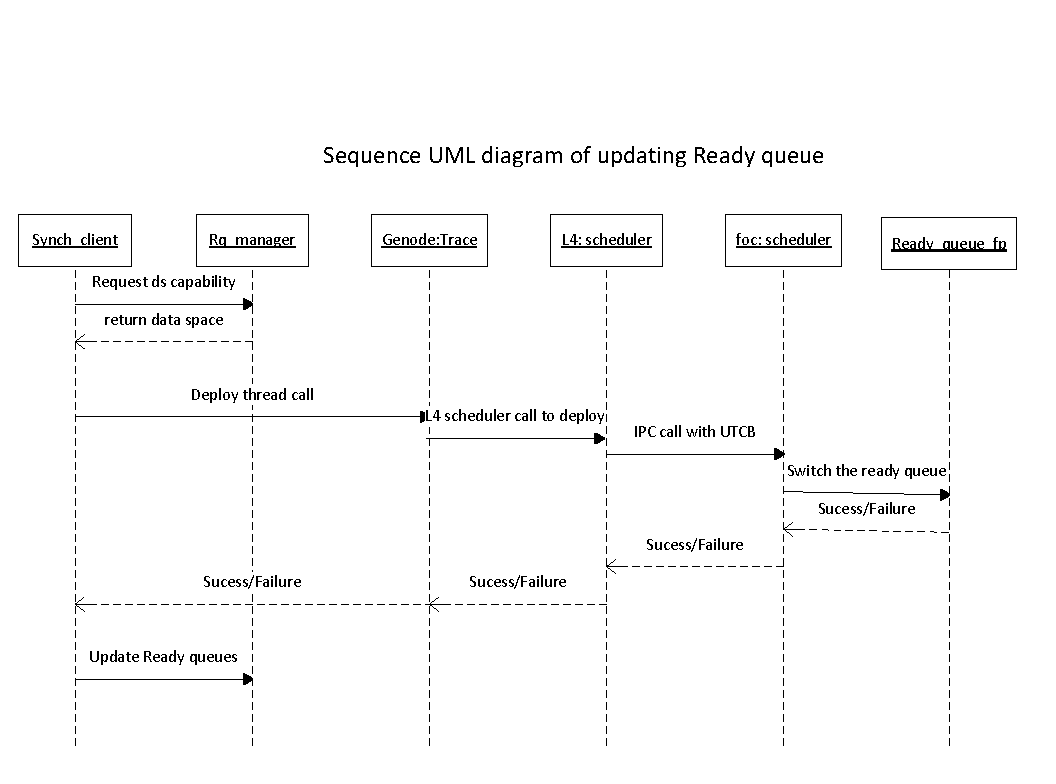
\includegraphics[width=1.0\linewidth]{figures/sequence_classUpdate}
\caption{Sequence diagram of updating ready queue from the Genode component}
\label{fig:sequence_classUpdate}
\end{figure}

%TODO explain the sequence diaram here
%TODO Add articles
%TODo remove commas from figure

\section{Rq\_manager module}

 The class \texttt{Rq\_manager} is the driver class of this component. It creates and maintains multiple ready queues at the user-level component, where each queue is of type Rq\_buffer. The Rq\_buffer is a template class, which implements a circular array by using the Genode dataspace. Each entry in the Genode dataspace is a circular array of type Rq\_task struct, which represents a Genode thread.

The code listing \ref{rqmanager} shows the implementation of \texttt{Rq\_manager} class. The constructor of \texttt{Rq\_manager} class first gets the number of available cores from Monitoring agent, then the \texttt{\_init\_rq()} function initializes the ready queues by using \texttt{init\_w\_shared\_ds} method from the Rq\_buffer class. The \texttt{Rq\_manager} provides enqueue and dequeue operations for the manipulation of ready queue.

\begin{lstlisting}[caption={Rq\_manager class},label={rqmanager}, style=customcpp]
class Rq_manager
{	

		private:

			int _num_cores = 0;
			Rq_buffer<Rq_task> *_rqs; /* array of ring buffers (Rq_buffer with fixed size) */
			
			int _set_ncores(int);

		public:

			int enq(int, Rq_task);
			int deq(int, Rq_task**);
			int get_num_rqs();
			Genode::Dataspace_capability get_core_rq_ds(int);

			Rq_manager()
			{
				PINF("Value of available system cores not provided -> set to 2.");

				_set_ncores(2);
				_init_rqs(100);
			}

			_init_rqs(int rq_size)
			{

				_rqs = new Rq_buffer<Rq_task>[_num_cores];

				for (int i = 0; i < _num_cores; i++) {
					_rqs[i].init_w_shared_ds(rq_size);
				}
				Genode::printf("New Rq_buffer created. Starting address is: %p.\n", _rqs);

				return 0;

			}
}
\end{lstlisting}

The Rq\_buffer is a template class, which represents the ready queue in the application side. It implements a circular array with fixed size. It uses \texttt{head} pointer, which points to the beginning of the array and \texttt{tail} pointer, which points to the end of the array. The elements are always inserted at tail pointer and removed from head. The pointers are wrapped around, whenever they reach the end of the array. The free space available between head and tail is represented by using a pointer called \texttt{window}. 

Rq\_buffer has enqueue and dequeue functionalities which can be called from \texttt{Rq\_manager} to insert or remove an element from ready queue. It also provides a functionality to initialize and create a shared dataspace. The code listing \ref{rqbuffer} shows, memory allocation for the shared dataspace and attaching it to the RM session of the component.

\begin{lstlisting}[caption={Allocating dataspace},label={rqbuffer}, style=customcpp]

	Genode::Dataspace_capability _ds; /* dataspace capability of the shared object */
	char *_ds_begin = nullptr;        /* pointer to the beginning of the shared dataspace */

		/* 
		 * create dataspace capability, i.e. mem is allocated,
		 * and attach the dataspace (the first address of the
		 * allocated mem) to _ds_begin. Then all the variables
		 * are set to the respective pointers in memory.
		 */
	_ds = Genode::env()->ram_session()->alloc(ds_size);
	_ds_begin = Genode::env()->rm_session()->attach(_ds);

\end{lstlisting}

The code listing \ref{rqtask} shows the Rq\_task structure which represents an entry in the ready queue buffer. It contains the parameters such as task\_id to identify a Genode task.

\begin{lstlisting}[caption={Rq\_task structure},label={rqtask}, style=customcpp]
 struct Rq_task
 	{
 
			unsigned long task_id;
 			int wcet;
 			bool valid;
 
 	};
\end{lstlisting}

The access to this shared dataspace must be synchronized since both the \texttt{Controller} and the \texttt{Synch\_client} use  it. This is done by locks provided from Genode.

\section{Synch\_client module}
The \texttt{Synch\_client} class represents a Genode component which controls the process of scheduler ready queue update. It acts as a client in Genode by using the services of the \texttt{Rq\_manager} and accesses the shared dataspace. The \texttt{Controller} and the \texttt{Synch\_client} interaction is that of a producer-consumer relationship. The producer (\texttt{Controller}) decides and produces(puts it in a buffer) a thread that needs to be executed and consumer(\texttt{Synch\_client}) picks the threads to the kernel ready queue.

%TODO insert flowchart
The initial communication with the \texttt{Rq\_manager} is governed by RPC call. In order to make an RPC call, it creates a Connection object. As explained before there are a number of pointers used for manipulating the circular buffer. The different pointers used are:

\begin{labeling}{pointers}
	\item [\_rqbufp] Hold the pointer to the Rq\_buffer type
	\item [\_lock] Lock needed to ensure mutual exclusion
	\item [\_head] Head pointer, points to the start of Rq\_buffer
	\item [\_tail] Tail pointer, points to end of Rq\_buffer
	\item [\_window] The window of free spaces available in between head and tail
\end{labeling}
 
There can be more than one ready queue. So, we need multiple pointers of each type. The data type \texttt{vector} is used to represent the pointers as the available number of ready queues is unknown at the creation time. The declaration of all the data structures can be seen in the listing \ref{synchdata}. 

\begin{lstlisting}[caption={Data structures used in Synch\_client},label={synchdata}, style=customcpp]
	Rq_manager::Connection rqm;
	
	/* using vectors since we dont know the size initially */
	std::vector<int *> _rqbufp;
	std::vector<int *> _lock;
	std::vector<int *> head; 
	std::vector<int *> tail; 
	std::vector<int *> window;
	
	std::vector<Dataspace_capability> dsc;
	std::vector<Rq_manager::Rq_task*> buf;
\end{lstlisting}

We can use the Connection object created to make RPC calls to the\texttt{Rq\_manager}. The first RPC call is to obtain the number of ready queues available. For each ready queue available, it has to make an RPC call to get the dataspace capability and attach to the local RM session and initialize all the pointers shown in the listing \ref{synchdata}. 

After everything has been initialized the \texttt{Synch\_client} runs in an infinite loop. For each ready queue it tries to obtain the lock, if the locking is successful then it schedules the threads available in the ready queue. The infinite loop has two goals. First, it has to ensure that it moves on to the next ready queue so that the threads in other queues also gets scheduled. Second, is to reduce the amount of time spent in the critical section as little as possible. In order to achieve the above mentioned goals, the ids of the threads/tasks are copied to a local buffer, head and tail pointers updated and the lock is released. By this way the scheduling of threads by calling of Genode API is kept outside the critical section.

One more option to reduce the critical section is to have separate threads working on each of the ready queues. Each thread will be working on a different ready queue and there is no shared data between these thread, which guarantees the second goal mentioned for the infinite loop. 
 
\section{Ready queue update Mechanism}

The ready queue update mechanism follows the series of calls which are shown in sequence diagram \ref{fig:sequence_classUpdate}. The following subsections explain the implementation of the modules described in \ref{design:rqupdate}.

\subsection{Genode code changes}

Genode should provide a way to the application for calling the L4 API calls. In the present Genode code the L4 APIs calls for scheduling threads are done from \texttt{Platform\_thread.cpp}, where the thread gets created. But the \texttt{Platform\_thread} is not accessible from the application, as it doesn't provide any RPC interface for applications to make use of its services. The only way that the components communicate in Genode is by using RPC calls. So an RPC call needs to be provided for the components to use it. As of now this call is kept in \texttt{Trace} service. The trace service is being used by the monitoring agent already to obtain the data from the Genode. The Trace service has been extended to provide an API, which can be used to from the \texttt{Synch\_client} component.

The \texttt{base/src/trace/trace\_session\_component.cc} contain the API definition, in which it takes a structure argument of threads and calls the L4 scheduler call.

\subsection{L4 API calls} \label{imp:l4api}
I introduced a new L4 API which can be called from the Genode. The APi takes the following arguments:

\begin{itemize}
\item l4\_cap\_idx\_t: It takes a kernel object which is scheduler object.  

\item l4\_sched\_thread\_list: This is a structure which can be seen in \ref{l4api}, which has an array to hold the list of threads and the priorities for the same threads. 

\end{itemize}

The code listing  \ref{l4api} shows the l4\_sched\_thread\_list structure and the L4 API call which is called from Genode and this code is in \texttt{foc/l4/l4sys/scheduler.h}.
\begin{lstlisting}[caption={L4 scheduler API in scheduler.h},label={l4api}, style=customcpp]

typedef struct l4_sched_thread_list
{
	l4_cap_idx_t list[10];
	unsigned prio[10];
	int n;
}l4_sched_thread_list;

L4_INLINE l4_msgtag_t
l4_scheduler_deploy_thread(l4_cap_idx_t scheduler,
		l4_sched_thread_list thread) L4_NOTHROW
{
  return l4_scheduler_deploy_thread_u(scheduler, thread, l4_utcb());
}
\end{lstlisting}

The deploy thread function call has to fill the UTCB message registers and make an IPC call to the scheduler kernel object. The first register(mr[0]) is populated with the type of operation that the scheduler should do to with the information, in this case it is L4\_SCHEDULER\_DEPLOY\_THREAD\_OP. The second register is populated using a call to l4\_map\_obj\_control function, which returns a word. This word identifies the kernel objects, which come after this word in the message registers. After the map object control word, thread objects are filled in the message registers in the form of L4 flex pages. An L4 flex page represents a naturally aligned area of mappable space, such as memory, I/O-ports, and capabilities (kernel objects), in this case L4 flex represents thread object.
For each thread id which is sent an L4 flex page is created and stored in the UTCB message registers. The L4 API makes an IPC call to the kernel scheduler object. 

The code listing \ref{l4apimp} shows the L4 scheduler API implementation.

\begin{lstlisting}[caption={L4 scheduler API implementation},label={l4apimp}, style=customcpp]
L4_INLINE l4_msgtag_t
l4_scheduler_deploy_thread_u(l4_cap_idx_t scheduler, l4_sched_thread_list thread,
			  l4_utcb_t *utcb) L4_NOTHROW
{
  l4_msg_regs_t *m = l4_utcb_mr_u(utcb);
  m->mr[0] = L4_SCHEDULER_DEPLOY_THREAD_OP;
  m->mr[1] = l4_map_obj_control(0, 0);

  for(int i = 0; i < thread.n; i++){
	  m->mr[i+1] = l4_obj_fpage(thread.list[i], 0, L4_FPAGE_RWX).raw;
  }
  
  return l4_ipc_call(scheduler, utcb, l4_msgtag(L4_PROTO_SCHEDULER, thread.n+1, 1, 0), L4_IPC_NEVER);
  }
\end{lstlisting}
  
\section{Fiasco.OC code changes}
Fiasco.OC code changes are made in several files to incorporate the ready queue update mechanism in the kernel and following sections explain the code changes in each file.

\subsection{Scheduler.cpp}

The \texttt{l4\_ipc\_call} from the scheduler.h invokes \texttt{kinvoke} function. The first parameter of the UTCB is decoded to find out the operation that is involved in. The operation in this case was set to \texttt{deploy\_thread} and which calls the function \texttt{sys\_deploy\_thread}, which can be seen in code listing \ref{sysdeploycode}. It runs a for loop to get the number of available threads. The associated flex page is derived from the sent items and a look up is performed to obtain the thread objects. The thread objects can be used to obtain the scheduler context which they are associated with. The scheduler context objects are used to create ready queue list(Fp\_list). This list is used to switch the actual ready queue of the scheduler.

The specified ready queue of the CPU can be obtained if the CPU was specified from the \texttt{Controller} otherwise the ready queue of the threads home CPU can be used. The current implementation creates and works with fixed priority list, however, this can be extended easily to create the corresponding ready queue list. If there is only one thread the \texttt{ready\_enqueue} function can be called instead of exchanging the complete list.


\begin{lstlisting}[caption={Thread extraction and ready list creation},label=sysdeploycode, style=customcpp]
Scheduler::sys_deploy_thread(L4_fpage::Rights, Syscall_frame *f, Utcb const *utcb)
{
	printf("[Scheduler: sys_deploy_thread] 1\n");
	L4_msg_tag const tag = f->tag();
	Cpu_number const curr_cpu = current_cpu();

	Obj_space *s = current()->space();
	assert(s);

	typedef Sched_context::Fp_list List;

	List list;
	
	for(int i = 6 ; i <= tag.words(); i++){
				
				/*
				 *	Get the messages in an iterator
				 */
				L4_snd_item_iter snd_items(utcb, i);

				/*
				 * Check if the items exist
				 */
				if (EXPECT_FALSE(!tag.items() || !snd_items.next()))
					return commit_result(-L4_err::EInval);

				L4_fpage _thread(snd_items.get()->d);

				if (EXPECT_FALSE(!_thread.is_objpage()))
					return commit_result(-L4_err::EInval);

				/*
				 * Do a look up to get the corresponding thread and cast 
				 * it to Thread_object type
				 */
				Thread *thread = Kobject::dcast<Thread_object*>(s->lookup_local(_thread.obj_index()));
				if (!thread)
					return commit_result(-L4_err::EInval);

				printf("[Scheduler:sys_deploy] Thread to be scheduled: %lx\n", thread->dbg_id());

				list.push(thread->sched_context(), List::Front);

				Sched_context::Ready_queue &rq = Sched_context::rq.cpu(thread->home_cpu());

				if(i==tag.words()){
				 rq.switch_ready_queue(&list, 100);
				}
		}
}
\end{lstlisting}

\subsection{sched\_context-fp\_EDF.cpp}

This class implements the major functionalities to handle the ready queues. This class contains the lists of both FP ready queue and EDF ready queue and serves as a wrapper class to both type of lists. Any call made to access the either of the ready queue, goes through this class. The decision to call the specific ready queue function is made according to the type of the scheduler in use.

Since this work was involved with fixed priority lists, the check to find out the type of scheduler in use is not made and default is to use the FP ready queue. However, it can be extended easily to work with both the lists. Code listing \ref{switchrq} shows the calling of the function to fixed priority ready queue.

\begin{lstlisting}[caption={Exchanging the ready queue},label=switchrq, style=customcpp]
IMPLEMENT
bool
Sched_context::Ready_queue_base::switch_rq(Fp_list *list, unsigned prio)
{
	return fp_rq.switch_rq(list, prio);
}
\end{lstlisting}

\section{Synchronization method}\label{imp:sync}

The ready queue contains the scheduler contexts which belongs to the threads and which can run next. Modifying the ready queue list is a critical section and mutual exclusive access must be guaranteed. In a uniprocessor implementation this can work with the CPU lock, which disables the interrupts on the local CPU and no other threads will get CPU time in the middle of ready queue manipulation. For SMP systems the kernel must use a ready list local to the CPU and advantages of using the per CPU data is explained in the section \ref{foundations}. Fiasco.OC implements a per CPU variable which is used towards synchronization. When using per CPU variable the exclusive access to this variable is guaranteed by disabling the CPU preemption and once the access is finished the CPU preemption is enabled. By this way, if any CPU is in the middle of critical section, no thread is allowed to replace the current operation. 

The present method uses the per CPU variable method where it locks the CPU before exchanging the CPU list. The software transaction memory method was implemented but testing that method was a problem since using of SMT forces the GCC compiler required pthreads library to be present which was not possible to include to Fiasco.OC. The SMT method would eliminate the necessary to preempt the CPU since it executes all the exchange the instructions in one transaction.

A check is made in scheduler.cpp to find out if the ready queue is empty. If the ready queue is empty or it contains the idle thread then the immediate call is made to exchange the list. The static point in time method is to check if a thread from this ready list getting executed, if the thread is running
the exchange call waits till the scheduler takes the control back and thread list is exchanged. This is checked in the call from \texttt{schedule\_in\_progress} flag. 


\subsection{Ready\_queue\_fp.cpp}
Hereinafter the list that is sent is referred as new list and the list to be exchanged is referred as old list. Once the fixed priority ready queue is decided to be exchanged the new list and the priority is sent to the \texttt{switch\_rq} function from sched\_context-fp\_EDF class. It is assumed at this point that the new list contains the threads that are necessary to execute the threads, which include the idle thread, pager threads. The Fiasco.OC uses an idle thread which keeps the CPU busy when there are no threads are to be executed. The idle thread needs to be kept in the new list if it's not existing already. The old list can be used to identify the idle thread, which sits in the end of the old list. The pager thread is nece

The exchange of the list is a simple operation of changing the head pointers. The cyclic list is implemented in a file called \texttt{dlist}. I implemented a a function \texttt{exchange} which takes the list to be exchanged with the present list and sets the head of the old list to the new list. 

The listing \ref{rq_exchange} shows the \texttt{switch\_rq} function.

 \begin{lstlisting}[caption={Exchanging the ready queue},label=rq_exchange, style=customcpp]
 bool switch_rq(List *list, unsigned prio) {
   		assert_kdb(cpu_lock.test());
 
   		prio_next[prio].exchange(list);
 
   		//prio_next[prio].rotate_to(*++List::iter(list->front()));
 
   		typename List::BaseIterator it = List::iter(prio_next[prio].front());
   		dbgprintf("After exchange fp_rq: ");
   		do
   		{
   			dbgprintf("%lx => ",Kobject_dbg::obj_to_id(it->context()));
   		}while (++it != List::iter(prio_next[prio].front()));
   		dbgprintf("end\n");
 
   		return true;
   	}
 
\end{lstlisting} 

\section{Creating a new kernel object in Fiasco.OC}\label{implement:kernelobject}
In this section creating a new kernel object is explained, that can be utilized to make a dedicated work in the kernel. The following changes are required to create kernel object and compile it. A new class should be created, which inherits \texttt{Icu\_h<object name>} and
\texttt{Irq\_chip\_soft} classes. The class has to declare this as kernel object using a macro (FIASCO\_DECLARE\_KOBJ()) provided from Fiasco.OC and the memory is allocated outside the class by defining the kernel object and sending the class name as a parameter. The class has to have a static object created inside the class and an interrupt request(Irq\_base) object defined in it. In the constructor of the class it is important to register this object to initial kernel objects. 

The class definition and the registering of kernel object can be seen in listing \ref{kobject}. The new object is called \texttt{RQ\_manager}, which should take care of the ready queue handling.

\begin{lstlisting}[caption={Creating new kernel object},label=kobject, style=customcpp]
class RQ_manager : public Icu_h<RQ_manager>, public Irq_chip_soft
{
  FIASCO_DECLARE_KOBJ();
  typedef Icu_h<RQ_manager> Icu;

public:
  enum Operation
  {
	RQ_info = 0,
	Schedule_thread = 1,
  };

  static RQ_manager rq_manager;
private:
  Irq_base *_irq;
};

FIASCO_DEFINE_KOBJ(RQ_manager);

PUBLIC inline
RQ_manager::RQ_manager() : _irq(0)
{
  initial_kobjects.register_obj(this, 8);
}

PUBLIC
L4_msg_tag
RQ_manager::kinvoke(L4_obj_ref ref, L4_fpage::Rights rights, Syscall_frame *f,
                   Utcb const *iutcb, Utcb *outcb)
{
}

enum Protocol{
  Label_rq_manager = -22L,   // Protocol ID for rq manager objects<l4_types.cpp>
}
enum l4_msgtag_protocol{
L4_PROTO_RQ_MANAGER = -22L, //Protocol for messages to a rq_manager object<types.h>
}

static Cap_index const C_rq_manager = Cap_index(8); //kernel-thread-std.cpp
\end{lstlisting}

This class should implement few of the functions from the inherited classes such as \texttt{icu\_bind\_irq} and \texttt{icu\_set\_mode} and a \texttt{kinvoke} call which the Fiasco uses it to do interprocess communication.

This created kernel object needs to be associate with protocol ID. These protocol IDs are used for either
kernel implemented objects and this is assigned in the \texttt{l4\_types.h}, protocol section of the
l4\_msg\_tag and also it needs to be assigned with l4\_msgtag\_protocol. This kernel object is assigned a \texttt{Cap\_index} which it was registered against.